\documentclass[manuscript,screen]{acmart}


\IfFileExists{upquote.sty}{\usepackage{upquote}}{}
\IfFileExists{microtype.sty}{% use microtype if available
  \usepackage[]{microtype}
  \UseMicrotypeSet[protrusion]{basicmath} % disable protrusion for tt fonts
}{}
\makeatletter
\@ifundefined{KOMAClassName}{% if non-KOMA class
  \IfFileExists{parskip.sty}{%
    \usepackage{parskip}
  }{% else
    \setlength{\parindent}{0pt}
    \setlength{\parskip}{6pt plus 2pt minus 1pt}}
}{% if KOMA class
  \KOMAoptions{parskip=half}}
\makeatother

%%
%% This is file `sample-manuscript.tex',
%% generated with the docstrip utility.
%%
%% The original source files were:
%%
%% samples.dtx  (with options: `manuscript')
%% 
%% IMPORTANT NOTICE:
%% 
%% For the copyright see the source file.
%% 
%% Any modified versions of this file must be renamed
%% with new filenames distinct from sample-manuscript.tex.
%% 
%% For distribution of the original source see the terms
%% for copying and modification in the file samples.dtx.
%% 
%% This generated file may be distributed as long as the
%% original source files, as listed above, are part of the
%% same distribution. (The sources need not necessarily be
%% in the same archive or directory.)
%%
%%
%% Commands for TeXCount
%TC:macro \cite [option:text,text]
%TC:macro \citep [option:text,text]
%TC:macro \citet [option:text,text]
%TC:envir table 0 1
%TC:envir table* 0 1
%TC:envir tabular [ignore] word
%TC:envir displaymath 0 word
%TC:envir math 0 word
%TC:envir comment 0 0
%%
%%
%% The first command in your LaTeX source must be the \documentclass command.


% Options for packages loaded elsewhere
\PassOptionsToPackage{unicode}{hyperref}
\PassOptionsToPackage{hyphens}{url}
\PassOptionsToPackage{dvipsnames,svgnames,x11names}{xcolor}

\IfFileExists{bookmark.sty}{\usepackage{bookmark}}{\usepackage{hyperref}}

%% PANDOC PREAMBLE BEGINS


\providecommand{\tightlist}{%
  \setlength{\itemsep}{0pt}\setlength{\parskip}{0pt}}\usepackage{longtable,booktabs,array}
\usepackage{calc} % for calculating minipage widths
% Correct order of tables after \paragraph or \subparagraph
\usepackage{etoolbox}
\makeatletter
\patchcmd\longtable{\par}{\if@noskipsec\mbox{}\fi\par}{}{}
\makeatother
% Allow footnotes in longtable head/foot
\IfFileExists{footnotehyper.sty}{\usepackage{footnotehyper}}{\usepackage{footnote}}
\makesavenoteenv{longtable}
\usepackage{graphicx}
\makeatletter
\def\maxwidth{\ifdim\Gin@nat@width>\linewidth\linewidth\else\Gin@nat@width\fi}
\def\maxheight{\ifdim\Gin@nat@height>\textheight\textheight\else\Gin@nat@height\fi}
\makeatother
% Scale images if necessary, so that they will not overflow the page
% margins by default, and it is still possible to overwrite the defaults
% using explicit options in \includegraphics[width, height, ...]{}
\setkeys{Gin}{width=\maxwidth,height=\maxheight,keepaspectratio}
% Set default figure placement to htbp
\makeatletter
\def\fps@figure{htbp}
\makeatother

\definecolor{mypink}{RGB}{219, 48, 122}
\makeatletter
\@ifpackageloaded{caption}{}{\usepackage{caption}}
\AtBeginDocument{%
\ifdefined\contentsname
  \renewcommand*\contentsname{Table of contents}
\else
  \newcommand\contentsname{Table of contents}
\fi
\ifdefined\listfigurename
  \renewcommand*\listfigurename{List of Figures}
\else
  \newcommand\listfigurename{List of Figures}
\fi
\ifdefined\listtablename
  \renewcommand*\listtablename{List of Tables}
\else
  \newcommand\listtablename{List of Tables}
\fi
\ifdefined\figurename
  \renewcommand*\figurename{Figure}
\else
  \newcommand\figurename{Figure}
\fi
\ifdefined\tablename
  \renewcommand*\tablename{Table}
\else
  \newcommand\tablename{Table}
\fi
}
\@ifpackageloaded{float}{}{\usepackage{float}}
\floatstyle{ruled}
\@ifundefined{c@chapter}{\newfloat{codelisting}{h}{lop}}{\newfloat{codelisting}{h}{lop}[chapter]}
\floatname{codelisting}{Listing}
\newcommand*\listoflistings{\listof{codelisting}{List of Listings}}
\makeatother
\makeatletter
\makeatother
\makeatletter
\@ifpackageloaded{caption}{}{\usepackage{caption}}
\@ifpackageloaded{subcaption}{}{\usepackage{subcaption}}
\makeatother
%% PANDOC PREAMBLE ENDS

\setlength{\parindent}{10pt}
\setlength{\parskip}{0pt}

\hypersetup{
  pdftitle={Raising the Role of Vocabulary Hubs for Semantic Data Interoperability in Dataspaces},
  pdfauthor={Robert David; Vladimir Alexiev; Petar Ivanov},
  colorlinks=true,
  linkcolor={blue},
  filecolor={Maroon},
  citecolor={Blue},
  urlcolor={red},
  pdfcreator={LaTeX via pandoc, via quarto}}

%% \BibTeX command to typeset BibTeX logo in the docs
\AtBeginDocument{%
  \providecommand\BibTeX{{%
    Bib\TeX}}}

%% Rights management information.  This information is sent to you
%% when you complete the rights form.  These commands have SAMPLE
%% values in them; it is your responsibility as an author to replace
%% the commands and values with those provided to you when you
%% complete the rights form.
\setcopyright{acmcopyright}
\copyrightyear{}
\acmYear{}
\acmDOI{}

%% These commands are for a PROCEEDINGS abstract or paper.
\acmConference[]{}{}{}
\acmPrice{}
\acmISBN{}

%% Submission ID.
%% Use this when submitting an article to a sponsored event. You'll
%% receive a unique submission ID from the organizers
%% of the event, and this ID should be used as the parameter to this command.
%%\acmSubmissionID{123-A56-BU3}

%%
%% For managing citations, it is recommended to use bibliography
%% files in BibTeX format.
%%
%% You can then either use BibTeX with the ACM-Reference-Format style,
%% or BibLaTeX with the acmnumeric or acmauthoryear sytles, that include
%% support for advanced citation of software artefact from the
%% biblatex-software package, also separately available on CTAN.
%%
%% Look at the sample-*-biblatex.tex files for templates showcasing
%% the biblatex styles.
%%

%%
%% The majority of ACM publications use numbered citations and
%% references.  The command \citestyle{authoryear} switches to the
%% "author year" style.
%%
%% If you are preparing content for an event
%% sponsored by ACM SIGGRAPH, you must use the "author year" style of
%% citations and references.
%% Uncommenting
%% the next command will enable that style.
%%\citestyle{acmauthoryear}


%% end of the preamble, start of the body of the document source.
\begin{document}


%%
%% The "title" command has an optional parameter,
%% allowing the author to define a "short title" to be used in page headers.
\title{Raising the Role of Vocabulary Hubs for Semantic Data
Interoperability in Dataspaces}

%%
%% The "author" command and its associated commands are used to define
%% the authors and their affiliations.
%% Of note is the shared affiliation of the first two authors, and the
%% "authornote" and "authornotemark" commands
%% used to denote shared contribution to the research.


  \author{Robert David}
  \orcid{0000-0002-3244-5341}
            \affiliation{%
                  \institution{The Semantic Web Company}
                                                  \country{Austria}
                      }
        \author{Vladimir Alexiev}
  \orcid{0000-0001-7508-7428}
    \author{Petar Ivanov}
  \orcid{0000-0001-8448-1005}
            \affiliation{%
                  \institution{Ontotext}
                                                  \country{Bulgaria}
                      }
      

%% By default, the full list of authors will be used in the page
%% headers. Often, this list is too long, and will overlap
%% other information printed in the page headers. This command allows
%% the author to define a more concise list
%% of authors' names for this purpose.
%\renewcommand{\shortauthors}{Trovato et al.}
%%  
%% The abstract is a short summary of the work to be presented in the
%% article.
\begin{abstract}
Dataspaces are an important enabler for industrial sharing data (either
commercially licensed or private). Europe is investing heavily into
sectoral dataspaces, federation and orchestration platforms like SIMPL,
Eclipse DSC, GXFS, etc. Still, dataspaces enable shared data access, but
do not solve the data interoperability problem. For that, the consumer
would like to see the data from different providers in a harmonized and
semantically integrated form. The Vocabulary Hub service (part of the
IDSA RAM) provides a repository for ontologies and vocabularies. We
describe an approach of raising the role of the vocabulary hub to also
allow richer metadata description (e.g.~the meaning of every column in a
tabular dataset), and binding semantic descriptions to ingested
datasets, thus providing on-the-fly data semantization and easing data
querying. This is achieved through the integration of two commercial
semantic products (PoolParty and GraphDB), leveraging the partnership
between the Semantic Web Company and Ontotext, and is being developed
within the frame of the Digital Europe project UNDERPIN, with
applications to refinery and wind farm data.    
\end{abstract}

%%
%% The code below is generated by the tool at http://dl.acm.org/ccs.cfm.
%% Please copy and paste the code instead of the example below.
%%

%%
%% Keywords. The author(s) should pick words that accurately describe
%% the work being presented. Separate the keywords with commas.
\keywords{dataspaces, semantic interoperability, semantic
technologies, ontologies, vocabulary hub, oil and gas, renewable
energy, refineries, windfarms}


%%
%% This command processes the author and affiliation and title
%% information and builds the first part of the formatted document.
\maketitle

\setlength{\parskip}{-0.1pt}

\section{Introduction}\label{introduction}

The European data economy heavily depends on the availability of data
and the technological foundation to make use of it. Different industries
and communities can benefit mutually by sharing data with each other,
thereby supporting their digitization business goals. Machine-learning
systems heavily rely on high volumes of high-quality training data.
Examples are the well-known mobility dataspace and use cases like energy
communities for running simulations. To cope with the challenge of data
sharing, Dataspace approaches like the IDS RAM were introduced to not
only solve the technical aspects of data sharing, but also to establish
methods for data sovereignty so that dataspace participants can
determine themselves how and when others can make use of their data.

For making use of shared data, interoperability is a crucial factor.
While syntactic data exchange is well covered by clearly defined data
formats, there is still the open challenge of semantic interoperability.
IDS RAM is firmly based on semantic metadata for all aspects and actors
of a dataspace. Furthermore, it can leverage semantic interoperability
approaches through the Vocabulary Hub that stores ontologies and
semantic thesauri for data descriptions and can dereference URIs to
provide semantic details of data assets.

In this paper, we present our proposal for a technological solution of
an IDS Vocabulary Hub built on the integration of the GraphDB semantic
graph database and PoolParty Semantic Suite. We not only cover the core
Vocabulary Hub functionalities and responsibilities in a dataspace, but
also extend the idea towards a Semantic Layer for dataspaces, which
provides even more services to easily and semi-automatically manage
semantic interoperability. Thus we raise the role of the Vocabulary Hub
to not only store semantic assets, but also to bind semantic
descriptions dynamically to incoming data, therefore enabling richer
discovery and semantic data integration between datasets.

\section{Projects and Use Cases}\label{projects-and-use-cases}

In the expanding data economy landscape supported by dataspaces, we are
working on several projects which address practical data sharing needs
and where we experience the importance of semantic interoperability to
fulfill various use cases. Our solution is developed with main focus on
the \href{https://underpinproject.eu/}{UNDERPIN} project with use cases
of refineries and wind farms, but other projects, such as
\href{https://databri-x.eu/}{DataBri-X} provide use cases which were
considered.

\subsection{Manufacturing/Maintenance
Dataspace}\label{manufacturingmaintenance-dataspace}

Operating refineries and wind farms involves high maintenance costs.
Predicting potential failures and optimizing the maintenance operations
to minimize the costs can be business-critical. For establishing
predictive maintenance, we need large amounts of high quality training
data that can be obtained by data consolidation across different
refinery and wind farm measurement sources.

The UNDERPIN project addresses this problem by creating a dataspace for
European manufacturers in the refinery and renewable energy domains and
various SMEs across their value-chain ecosystem, such as equipment
suppliers. Extensive time series data is exchanged, but their format and
meaning is not standardized. Describing the meaning of these time series
facilitates semantic interoperability between datasets from different
providers. This description includes measured variable, quantity kind
and unit of measure, which sensor took the measurements, what it is
attached to, the detailed model and connectivity of that industrial
equipment.

\subsubsection{The Refinery Dataspace}\label{the-refinery-dataspace}

Refineries can be optimized regarding costs and efficiency by
considering not only individual components, but the production chain as
a connected system. In this use case, we aim to improve the maintenance
process as well as the decision making for preventive maintenance so as
to minimize the downtime and the impact on the production capabilities.

\subsubsection{The Wind Farm Dataspace}\label{the-wind-farm-dataspace}

Operating wind farms involves high costs for maintaining the wind
turbines. Predicting potential failures and optimizing the maintenance
operations to minimize the costs can be business critical. For
establishing predictive maintenance, we need large amounts of high
qualitative training data, which can be achieved by consolidating
different wind farm measurement sources. This use case provides
different kinds of tabular data, where consolidation needs semantic
harmonization of data.

\subsection{Energy and Legal
Dataspace}\label{energy-and-legal-dataspace}

Beyond the UNDERPIN project as the main use case provider, we also
consider use cases from other projects. We present 2 examples from the
DataBri-X project, which work on different content types of data and
have different usage scenarios. We considered these as well when
designing our solution to make it applicable to a broader range of use
cases.

\subsubsection{The Energy Dataspace}\label{the-energy-dataspace}

In this use case, we run simulations for energy communities, which
predict the behavior of the energy grid. To provide precise predictions,
there is the need of high amounts of example data. This data is of
numeric type and different tabular data sources need to be semantically
consolidated.

\subsubsection{The Legal Dataspace}\label{the-legal-dataspace}

Analyzing documents in the legal domain is a highly challenging task
because of the complexity of legal information. We provide recommender
services for insights into corpora of legal documents that identify the
meaning via a legal knowledge graph, NLP analysis and semantic
annotations.

\subsection{The Problem}\label{the-problem}

``Standard'' dataspace solutions provide access to data and metadata
descriptions, but they do not typically address the data integration
problem. If a consumer wants to consume datasets from different
providers in an integrated way, they need to harmonize the data to some
common model, convert it, store it in a database, and potentially
implement entity linking (correlation of different records that are
about the same real-world thing) and data fusion.

Above we gave just 4 examples to illustrate the heterogeneity of data in
the context of different use cases. We aim to develop solutions that not
only fulfill the dataspace needs, but also improve the situation
regarding semantic interoperability by providing services that can be
easily leveraged to implement such use cases.

\section{Approach and IT-Solution}\label{approach-and-it-solution}

To tackle this problem, we introduce Semantic Web standards and
technologies to model and process data. Vocabularies and ontologies
(expressed using RDFS, OWL and SKOS) can represent data with a clear
semantics based on standards. We leverage GraphDB and PoolParty as two
software components that implement these standards to process the data.

\subsection{IDS Vocabulary Hub}\label{ids-vocabulary-hub}

In this paper, we focus on the IDSA approach to dataspaces. IDSA defines
the architecture of dataspaces in the reference architecture model
IDS-RAM (current version 4). One of the defined architectural
components, the Vocabulary Hub, has the role of providing vocabularies
to annotate and describe data assets and services. These vocabularies
form a common language to enable semantic interoperability among the
dataspace participants. The Vocabulary Hub is responsible for resolving
annotations of data assets and for providing details in the form of
standardized semantic descriptions. It supports the use of Semantic Web
standards for defining and representing RDF vocabularies and ontologies
and thereby provides semantic interoperability in a standardized and
machine-readable way.

\subsection{GraphDB Graph Database}\label{graphdb-graph-database}

TODO

\subsection{PoolParty Semantic Suite}\label{poolparty-semantic-suite}

PoolParty Semantic Suite is a semantic middleware platform based on W3C
standards, specifically the Semantic Web, which provides a wide variety
of functionality in the area of knowledge graph management, graph-based
NLP, semantic search and recommender systems.

At the core of PoolParty is the Thesaurus Manager, which can be used to
create and maintain RDF-based vocabularies, including ontologies,
schemas and different kinds of knowledge models. These vocabularies can
be applied for various use cases, from bridging data silos in
enterprises by implementing data consolidation via the vocabularies, to
annotating documents with semantic annotations to implement semantic
search and recommendations which provide insights into data.

PoolParty is well suited to form the basis of a vocabulary management
system within a dataspace, effectively implementing not only the
Vocabulary Hub role, but also providing additional services that improve
the expressiveness of common vocabularies and automate semantic
interoperability.

\subsection{The GraphDB Poolparty
Integration}\label{the-graphdb-poolparty-integration}

The integration of GraphDB and PoolParty leverages synergies of a
high-performance graph database with a platform for knowledge graph
management.

Both GraphDB and PoolParty are based on W3C recommendations like RDF,
OWL and SPARQL. They therefore seamlessly integrate with each other, but
also with other services and components in dataspaces which support
these machine-readable standards for semantic interoperability.

\section{A Semantic Solution and its
Benefits}\label{a-semantic-solution-and-its-benefits}

When harmonizing data, we need to provide a method to automatically map
and process it, so this can be done efficiently on large datasets and/or
regular updates in dataspaces. The benefit provided should support the
ML training in such a way that the consolidated dataset is exposed as a
uniform training dataset.

\subsection{Semantic Layer Approach}\label{semantic-layer-approach}

The Vocabulary Hub, as IDS defines it in the IDS-RAM, is a basic
building block to achieve semantic interoperability in dataspaces by
provisioning common vocabularies. We aim to go one step further and
envision a Semantic Layer for dataspaces, which provides
vocabulary-based services for advanced and automated semantic
descriptions of metadata and data. The Semantic Layer is implemented as
services based on the GraphDB and PoolParty and provided as a one
seamlessly integrated component.

In the following, we discuss i) the services provided for the Vocabulary
Hub component and ii) additional services as Vocabulary Hub extensions
that implement a Semantic Layer for dataspaces.

Vocabulary Hub Services: - RDF based: both GraphDB and PoolParty store
and manage data based on the RDF data model. RDF is the basic building
stone and underlying vocabulary definitions. - Scalable vocabulary
storage: cluster implementation for higher throughput and a fault
tolerant architecture. - Knowledge graph management: easy management of
vocabularies using a rich web user interface and integration via Web
APIs. Vocabularies can be created and edited based on standards like
RDFS, OWL and SKOS, and existing vocabularies can be reused and combined
to fit specific dataspace needs. - SPARQL service for semantic lookups:
dereference URIs describing data assets to retrieve a semantic
description of the entity from the graph database.

Semantic Layer Services support both unstructured and structured data
assets: - Unstructured data: semantic annotation services for documents
based on concept tagging. PoolParty's KG-based NLP primarily uses SKOS
taxonomies to identify concepts in documents, but can be extended with
OWL ontology elements (classes, properties) for increased
expressiveness. - Structured data: we support structured data
harmonization methods, including semantic mapping and linking SKOS
concepts - Ontology-Based Data Access (OBDA) is used for virtualization
of relational data, i.e.~accessing relational data as semantic data. It
is well suited for semantic querying of large amounts of data, while
keeping the original relational data in place (NoETL approach).
Ontologies are leveraged to construct the OBDA mapping; they are
governed via the Semantic Layer and can harmonize data assets of various
formats using a precise mapping. Furthermore, it can be used to
establish a fine-grained access control, thereby deciding for individual
data elements if they should be exposed ot not. - RDB to RDF Mapping
Language (R2RML) \citep{souripriyadasR2RMLRDBRDF2012} and RDF Mapping
Language (RML) \citep{RMLIntroduction2024} are intended for data
transformation processes within a dataspace, where the original source
is used as a basis to create an RDF representation (ETL approach). -
GraphDB supports both OBDA and R2RML through its integration of ONTOP
\citep{bagosiOntopFrameworkOntology2014}. The same mappings can be used
for NoETL virtual data access, or for ETL (to materialize the semantic
data). - CSV on the Web (CSVW) \citep{swirrlCSVWStandards2024} is a set
of W3C standards that allow detailed semantic description of tabular
data using a JSON ``manifest'' file. - SKOS concepts are used for
structured data in several ways. Concepts can be directly added to RDF
data via semantic links (properties from an ontology), they can be used
to annotate specific literals of an RDF graph, or they can be used to
associate documents with (specific parts of) an RDF graph. - Inference
services: we provide metadata expansion services based on interlinked
vocabularies in combination with ontologies. This inference approach can
be used with semantic tagging for unstructured data, as well as the
structured data approaches. - Inference tagging is provided by a
PoolParty tagging service in combination with an expansion query for
implementing the inference. The query can be configured to work for
various scenarios. - Vocabulary crosswalks are a data modeling approach
using interlinks to relate: - Different vocabularies from similar or the
same domain that cover different areas or aspects of the domain. By
relating concepts with each other using 1:1, 1:n and m:n relations, we
can automatically expand queries and annotations by traversing the
interlinked graph. - Different versions of the same vocabulary to
automatically translate between those versions. - Metadata inference
based on interlinked vocabularies is similar to crosswalks, but intended
to represent different levels of abstraction, so that we are able to
infer from a more general vocabulary to a more specific vocabulary and
vice versa. For example, we can start with DCAT themes vocabularies and
link to further vocabularies, which are more specific for certain areas
or which go into more detail.

\subsection{Software Architecture}\label{software-architecture}

The following figure shows the architecture of our approach:

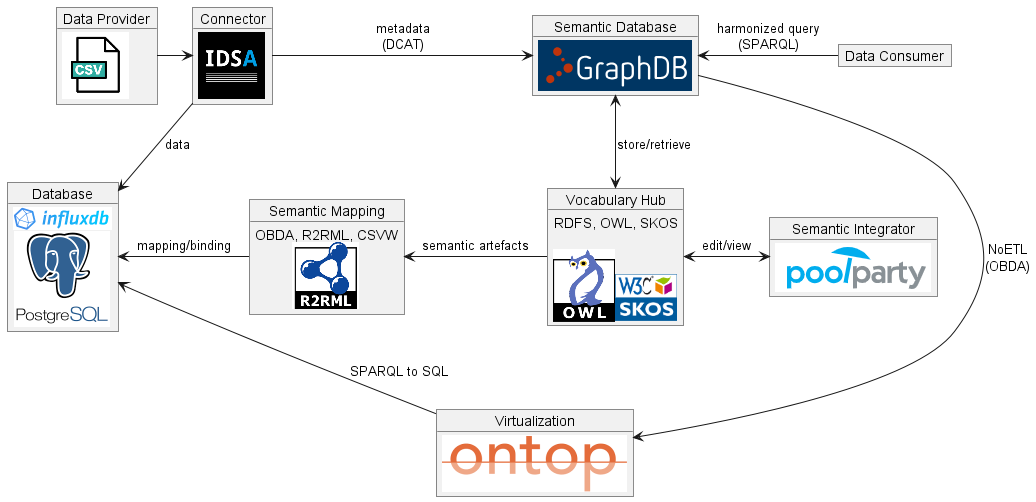
\includegraphics{img/architecture.png}

\begin{itemize}
\tightlist
\item
  A Data Provider sends data through the Connector, and at the same time
  provides basic metadata (DCAT)
\item
  Selected data can be stored in Database(s) managed by the dataspace,
  for easier access and querying.

  \begin{itemize}
  \tightlist
  \item
    For large-volume time series data, we recommend to use InfluxDB,
    PostgreSQL, Google BigQuery, etc.
  \item
    Of course, access control is very important here. We'll leverage
    GraphDB's
    \href{https://graphdb.ontotext.com/documentation/10.6/fine-grained-access-control.html}{Fine-grained
    Access Control}, but access control in the time series database is
    also important.
  \item
    Depending on Provider preferences and agreements, other data may
    stay at the source, and be delivered to the Consumer only
    dynamically through the Connector.
  \end{itemize}
\item
  The Vocabulary Hub stores relevant semantic assets: ontologies and
  thesauri. These are added based on relevant use cases and datasets,
  following a dataspace governance process.
\item
  The Vocabulary Hub also stores mapping assets, such as OBDA or R2RML
  mappings and CSVW manifests.
\item
  PoolParty Semantic Integrator is used to edit, view and manage the
  semantic assets, and to bind mapping assets to incoming data.
\item
  For virtual access to relational data, ONTOP is used to translate
  SPARQL to SQL dynamically and to convert returned data to SPARQL
  result format.
\item
  The Data Consumer benefits from:

  \begin{itemize}
  \tightlist
  \item
    More powerful dataset discovery by using richer semantic queries,
    e.g.

    \begin{itemize}
    \tightlist
    \item
      ``Give me all time series related to compressor C123'' (equipment
      instance)
    \item
      ``Give me all time series related to temperature'' (measured
      quantity)
    \item
      ``Give me all time series of bearings'' (equipment kind or machine
      part)
    \end{itemize}
  \item
    Harmonized querying of datasets from multiple providers.
  \end{itemize}
\end{itemize}

\section{Conclusion and Future Work}\label{conclusion-and-future-work}

We presented an approach for dynamically binding datasets to semantic
descriptions in a dataspace's Vocabulary Hub, therefore facilitating
data harmonization and easier data consumption. We have implemented a
first prototype of our approach, which builds on the integration of
GraphDB and PoolParty. As next steps, we will bring this solution into
use cases and into broader discussion to gain insight and develop it
further.

The next steps include: - Bringing it into actual dataspaces in
practice, representing and integrating datasets from different dataspace
participants. - Implementing use cases for richer discoverability,
harmonized querying and support for different content types of
structured and unstructured data. - Explore how ML can benefit regarding
quality in practice when providing consolidated and cleaned data via
dataspaces. - Discuss how we can extend the IDS-RAM with services to
improve the support for semantic interoperability provided by our
solution.

\section{Acknowledgements}\label{acknowledgements}

This work is partially supported by the Digital Europe programme project
\href{https://underpinproject.eu/}{UNDERPIN} (grant agreement 101123179)

\bibliographystyle{ACM-Reference-Format}
\bibliography{bibliography.bib}

%% begin pandoc before-bib
%% end pandoc before-bib
%% begin pandoc biblio
%% end pandoc biblio
%% begin pandoc include-after
%% end pandoc include-after
%% begin pandoc after-body
%% end pandoc after-body

\end{document}
\endinput
%%
%% End of file `sample-manuscript.tex'.
